%-----------------------------------------------------------
%-----------------------------------------------------------
%	Guide d'introduction à Java et WPILib
%	Par Étienne Beaulac
%	Ultime 5528
%	Mai 2017
%-----------------------------------------------------------
%-----------------------------------------------------------


\documentclass[12pt]{report}

%Code display, avant Babel !
%\usepackage{listings, minted}

\usepackage[francais]{babel}
\usepackage[utf8]{inputenc}
\usepackage[scaled]{helvet}
\renewcommand\familydefault{\sfdefault} 
%\usepackage{libertine}
%\usepackage{libertinust1math}
\usepackage[T1]{fontenc}
%\usepackage{lmodern}
%\usepackage{avant}

% Marges
\usepackage[margin=2cm]{geometry}

%Custom font sizes
\usepackage{anyfontsize}

%Tableau en français (et non table)
\usepackage{caption}
%\captionsetup[table]{name=Tableau}

%packages graphiques, mathématiques
\usepackage{amsfonts, amsmath, amssymb}

%Afficher des images avec includegraphics
\usepackage{graphicx}

% Tableaux extensibles
\usepackage{tabularx}
\usepackage{booktabs}

%Image avec caption
\newcommand{\image}[2]{%

}



%Virgule pour nombres français
%\usepackage{icomma}

%Liens hypertextes
\usepackage{hyperref}
\hypersetup{
    colorlinks=true,
    linkcolor=blue,
    filecolor=magenta,      
    urlcolor=blue,
}

%Couleurs
\usepackage{xcolor}
\definecolor{ultRed}{RGB}{190,30,45}
\definecolor{ec-red}{RGB}{237,28,36}
\definecolor{ec-orange}{RGB}{255,127,39}
\definecolor{ec-yellow}{RGB}{255,242,0}
\definecolor{ec-green}{RGB}{34,177,76}
\definecolor{ec-purple}{RGB}{163,73,164}

%\usepackage{eso-pic}

%Nice code snippets
\usepackage[chapter]{minted}
\setminted[java]{%
	linenos,
	autogobble
}

%Nice frames for minted
\usepackage{tcolorbox}
\tcbuselibrary{minted, skins, xparse, breakable}
\usepackage{tikz}
\usetikzlibrary{arrows.meta, shapes.geometric}

% Ne pas copier les numéros de lignes de code
\usepackage{accsupp}
\newcommand\emptyaccsupp[1]{\BeginAccSupp{ActualText={}}#1\EndAccSupp{}}
%default definition is: \def\theFancyVerbLine{\rmfamily\tiny\arabic{FancyVerbLine}}
\let\theHFancyVerbLine\theFancyVerbLine% don't apply our patch to hyperref's version
\def\theFancyVerbLine{\rmfamily\tiny\emptyaccsupp{\arabic{FancyVerbLine}}}


%Frame for commands
\newcommand{\commande}[1]{%
\tcbox[on line, size=fbox, colframe=black, boxrule=0.75pt, tcbox raise base]{#1} %boxsep=0pt, left=5pt, right=5pt, top=8pt, bottom=8pt
}

%inline code
%\usepackage{varwidth}
%\newcommand{\code}[1]{%
%\tcbox[on line, size=fbox, colframe=gray, boxrule = 0.25pt, tcbox raise base]{\texttt{#1}} %boxsep=0pt, left=5pt, right=5pt, top=8pt, bottom=8pt
%}

%Frame for minted listings
\newtcblisting[list inside=mybox, auto counter, number within=chapter]{MyTCB}[2][]{%
	colframe=ultRed,
	title={\textsc{Code \thetcbcounter} --- #2},
	sharp corners=south,
	boxsep=3mm,
	left=0.7cm,
	listing only,
	list text={#2},
	minted language=java,
	minted options={obeytabs, linenos, autogobble, baselinestretch=1, tabsize=4, breaklines=true}, #1}

%Frame for minted listings
\newtcblisting{code}[1][\linewidth]{%
	colframe=ultRed,
	sharp corners=all,
	boxsep=1mm,
	left=0.7cm,
	listing only,
	width = #1,
	minted language=java,
	minted options={linenos = false, autogobble, baselinestretch=1, tabsize=4}}


%Commande pour images inline
\newcommand{\inlinepic}[1]{%
  \begingroup\normalfont
  \includegraphics[height=1em]{#1}%\fontcharht\font`\B
  \endgroup
}

% Environnement console
\newenvironment{console}
	{
	\tcolorbox[title={Sortie console}, sharp corners = south, boxsep = 1.5mm]{} \tt
	}{\endtcolorbox}

%Listings caption
\renewcommand{\listingscaption}{Extrait de code}
\renewcommand{\listoflistingscaption}{Liste des extraits de code}

%Better aligned lists
\usepackage{scrextend}

%\usepackage{multirow}
%\usepackage{tikz}
%\usepackage{pgfplots}
%\pgfplotsset{width=7cm, compat=1.13}
%\usepgfplotslibrary{fillbetween}

%\setlength{\jot}{10pt} % Modifie l'espace entre les équations d'un bloc Align

%\showboxdepth=\maxdimen
%\showboxbreadth=\maxdimen


%Indentation nul au début de paragraphe
\setlength{\parindent}{0pt}

%Espace entre les paragraphes
\setlength{\parskip}{0.5\baselineskip}


%Espace entre les notes de bas de page
\setlength{\footnotesep}{0.95\baselineskip}



%----------------------------------------------------
%----------------------------------------------------
%----------------------------------------------------
% Début du document
%----------------------------------------------------
%----------------------------------------------------
%----------------------------------------------------

\begin{document}
%
%
%----------------------------------------------------
%----------------------------------------------------
% Page titre
%----------------------------------------------------
%----------------------------------------------------
%
%
\begin{titlepage}
	\vspace*{2.5cm}
	\hspace*{-2cm}\colorbox{ultRed}{%
	{\begin{minipage}{\paperwidth}	
		{\ \\[1cm] \hspace*{2cm} {\fontsize{40}{50}\selectfont Guide} \\[10pt]
		\hspace*{2cm} {\Large Formation Java et WPILib} \vspace*{1cm}}
	\end{minipage}}}\\[10pt]
	%
	\begin{minipage}{6cm}
		\raisebox{-0.1\height}{\parbox[b]{4cm}{\raggedleft {\large Étienne Beaulac\\[5pt] Ultime FRC 5528}\\[15pt] {\small Dernière modification\\ \today} }}%
		\hspace*{0.05\textwidth}%
		\raisebox{-0.5\height}{\rule{0.5pt}{6cm}}%
		\hspace*{0.32\textwidth}%
		\raisebox{-0.5\height}{
\includegraphics[trim={2.6cm 0 2.6cm 0}, clip, height=7cm]{logo_ultime.png}}%
	\end{minipage}
\end{titlepage}
\pagebreak
%
\thispagestyle{empty}
\strut
\newpage
%
% Enlever les hyperliens bleus
{\hypersetup{hidelinks}
%
\clearpage
\pagenumbering{roman}
\setcounter{page}{1}

\tableofcontents

\newpage
%
\tcblistof[\section*]{mybox}{Table des extraits de code}
\addcontentsline{toc}{chapter}{Table des extraits de code}
\newpage
%
\listoffigures
\addcontentsline{toc}{chapter}{Table des figures}
\newpage
%
\linespread{1.5}
\normalsize
\pagenumbering{arabic}
\setcounter{page}{1}
} % Fin hyperliens noirs


%----------------------------------------------------
% Ajouter fancyhf{}
%----------------------------------------------------

\part{Les bases de Java}

%----------------------------------------------------
%----------------------------------------------------
%----------------------------------------------------
% Chapitre 1 - Introduction au Java
%----------------------------------------------------
%----------------------------------------------------
%----------------------------------------------------
\chapter{Introduction au Java}
%
%
%----------------------------------------------------
% Section - Les langages de programmation
%----------------------------------------------------
%
\section{Les langages de programmation}
La programmation, en somme, est l'art de formuler ses algorithmes de manière à les faire comprendre à un ordinateur (Ada Lovelace, vers 1840\footnote{On attribue à Ada Lovelace, mathématicienne britannique, la création des premiers programmes informatiques. Ils furent conçus pour être exécutés sur la machine analytique de William Babbage, entièrement mécanique.}). Cependant, à la base, les ordinateurs ne comprennent que le binaire (Alan Turing, 1936\footnote{Alan Turing, mathématicien, cryptologue et logicien britannique, formalisa en 1936 le concept mathématique de \emph{machine de Turing}.}). Pour se simplifier la vie, les informaticiens ont créé des langages intermédiaires qui font le pont entre nous et les ordinateurs (Grace Hopper, 1951\footnote{Grace Hopper, informaticienne et \emph{rear admiral (lower half)} de l'armée américaine, conçut en 1951 \emph{A-0 System}, le premier compilateur pour ordinateur.}). Tous les langages de programmation ont le même but : vous permettre de parler à un ordinateur plus simplement qu'en binaire.
%
%
% Image - Processus de compilation
%
\begin{figure}[!htbp]
  \centering
  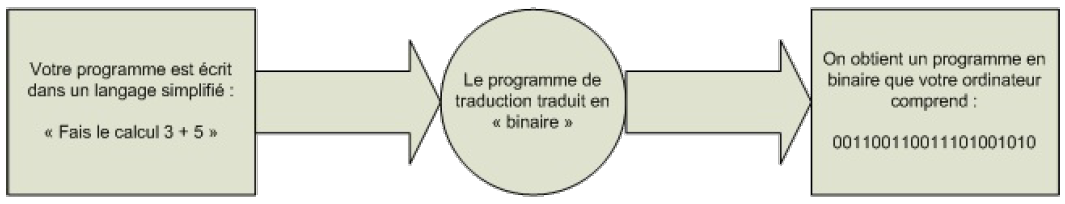
\includegraphics[width=0.9\textwidth]{compilation.png}
  \caption{Le processus de compilation.}
\end{figure}






%----------------------------------------------------
% Section - Qu'est-ce que le Java?
%----------------------------------------------------
%
\section{Qu'est-ce que le Java?}
%
%
Le langage Java a été créé , entre autres, par James Gosling, Patrick Naughton et Mike Sheridan, tous les trois employés chez \emph{Sun Microsystems} dans les années 1990. Sa première version parut en 1995. Java est maintenant propriété de \emph{Oracle Corporation}.

Java est un langage presque entièrement \textbf{orienté objet}. Il reprend une grande partie de la syntaxe du C/C++, tout en y ajoutant certaines fonctionnalités : une librairie standard très complète, la réflexivité, les expressions lambdas, l'\emph{autoboxing} et l'\emph{unboxing}, les interfaces, et plusieurs autres.  Toutefois, les pointeurs et l'héritage multiple ne sont pas supportés. Ils ajouteraient une trop grande complexité au langage, alors que le but de Java est d'être simple, sécuritaire et robuste.

Le Java compte un nombre impressionnant d'utilisateurs. Une de ses forces est d'ailleurs sa portabilité. Tout programme Java, une fois compilé en \emph{bytecode}, peut fonctionner sur n'importe quelle machine, tant qu'une machine virtuelle Java (JRE, ou \emph{Java Runtime Environment}) y est installée.




%--------------------------------------------------------
% Chapitre - Votre premier programme 
%--------------------------------------------------------
%
\chapter{Votre premier programme}

\textit{Manuel de référence : p. 1 à 22 et 33 à 38.}

%--------------------------------------------------------
% Section - Les environnements de développement intégré 
%--------------------------------------------------------
% TODO : Annexe A - Eclipse
%
\section{L'IDE Eclipse}
%
Pour programmer, il est préférable d'utiliser un bon environnement de développement (\textbf{IDE}, ou \emph{Integrated Development Environment}). De tels logiciels comprennent un \textbf{éditeur de texte}, un \textbf{compilateur} et un \textbf{débogueur}. Nous utiliserons l'IDE Eclipse\footnote{Pour plus d'information concernant Eclipse, consultez ...} avec l'extension WPILib fournie par FIRST.

Eclipse est disponible gratuitement sur \href{https://www.eclipse.org}{eclipse.org}. Vous devrez également vous assurer d'avoir installé une version récente du \href{http://www.oracle.com/technetwork/java/javase/downloads/index.html}{JDK} (\emph{Java Development Kit}). Les étapes d'installation sont également détaillées \href{http://wpilib.screenstepslive.com/s/4485/m/13809/l/599681-installing-eclipse-c-java}{ici}.

% Image - Interface principale de Eclipse
%
\begin{figure}[!htb]
  \centering
  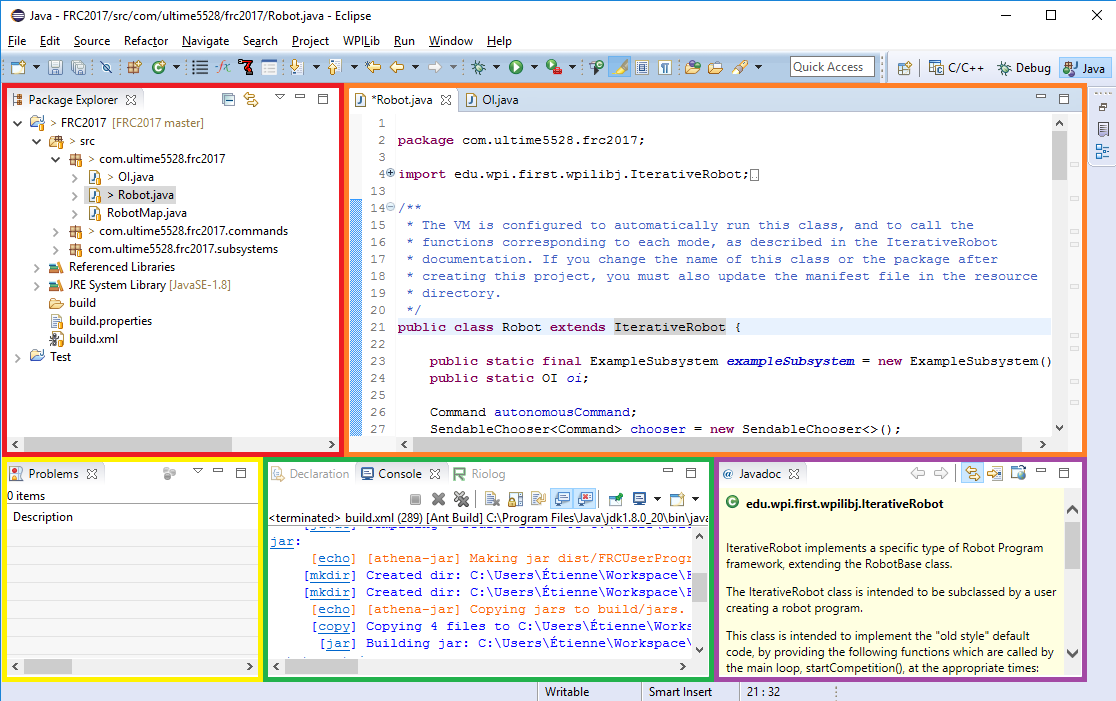
\includegraphics[width=\textwidth]{interface-eclipse.png}
  \caption{L'interface principale de Eclipse.}
\end{figure}
%
Eclipse est un logiciel ayant plusieurs fonctionnalités. On peut d'ailleurs lui en ajouter à l'aide d'extensions (\emph{plugins}), comme celle que nous utiliserons pour développer sur le roboRIO. Voici les fenêtres qui nous intéresserons le plus :

\begin{labeling}{\ Package Explorer\ }
%
\item[\colorbox{ec-red}{\emph{Package Explorer}}] Cette fenêtre regroupe tous vos projets, subdivisés en dossiers et paquetages (\emph{packages}), jusqu'aux fichiers Java.
%
\item[\colorbox{ec-orange}{Fenêtre d'édition}] Cette fenêtre affiche tous les fichiers que vous êtes en train d'éditer, vous permettant facilement de naviguer entre différents documents.
%
\item[\colorbox{ec-yellow}{\emph{Problems}}] Comme son nom l'indique, on y retrouve une liste de tous les avertissements et erreurs concernant votre code. Chaque item précise la nature de l'erreur et où elle se trouve.
%
\item[\colorbox{ec-green}{Console}] La console est un outil essentiel, c'est le premier lien entre vous et l'exécution de votre programme. Vous pourrez y afficher du texte et en insérer.
%
\item[\colorbox{ec-purple}{Javadoc}] Java a l'avantage de fournir son propre outil de documentation. Il suffit de cliquer sur un mot (classe, variable, méthode, etc.) et sa description y apparaîtra. Nous verrons plus loin comme créer ses propres entrées pour Javadoc.
\end{labeling}

Évidemment, toute l'interface est entièrement personnalisable. À vous de l'adapter comme il vous plaira!






%--------------------------------------------------------
% Section - Création du projet 
%--------------------------------------------------------
%
\section{Création du projet}
%
\begin{enumerate}
\item Dans Eclipse, créez un nouveau projet avec \commande{File > New > Java Project}. Donnez un nom à votre projet, puis cliquez sur \commande{Finish}.

\item Ajoutez une classe à votre projet : \commande{Clic droit sur votre projet > New > Class}. Donnez un nom à votre classe, cochez l'ajout de la méthode \commande{main}, puis cliquez sur \commande{Finish}.

\item Complétez le corps de la méthode avec l'exemple suivant, puis compilez et exécutez votre programme.
\end{enumerate}
%
% Code - Programme de base
%
\begin{MyTCB}{Programme de base}
public class MonPremierProgramme {

	public static void main(String[] args) {
	
		System.out.println("Hello, world");
		
	}
	
}
\end{MyTCB}
%
%
% Image - Compiler/Exécuter avec Eclipe
\begin{figure}[!htb]
	\centering
	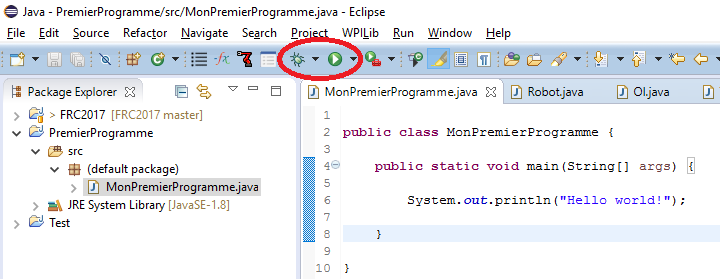
\includegraphics[width=\textwidth]{compilation-eclipse.png}
	\caption{Compiler, exécuter et déboguer un programme avec Eclipse.}
\end{figure}
%
Le bouton \inlinepic{debug-btn-eclipse.png} vous permet de lancer votre programme en mode débogage. La flèche verte \inlinepic{execute-btn-eclipse.png}, quant à elle, compile et exécute. Après avoir cliqué dessus, vous devriez voir apparaître du texte dans votre console.
%
% Image - Écriture console
%
\begin{figure}[!ht]
	\centering
	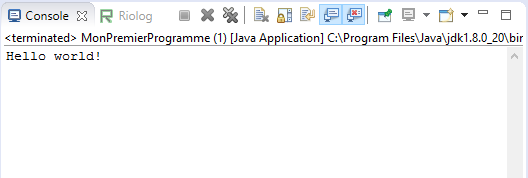
\includegraphics[scale=1]{ecriture-console.png}
	\caption{Écriture dans la console.}
\end{figure}

Félicitations, vous venez d'exécuter votre premier programme! Analysons en détail ce qu'il se passe à l'intérieur.






%--------------------------------------------------------
% Section - Instructions
%--------------------------------------------------------
%
\section{Les instructions}
En Java, une \textbf{instruction} est une commande effectuant une certaine action. On écrit une instruction par ligne, et chacune se termine toujours par un \textbf{point-virgule} (\ {;}\ ). Pour l'instant, votre programme ne contient qu'une instruction : 
\begin{code}
System.out.println("Hello, world!");
\end{code}
Vos instructions sont écrites dans la méthode \texttt{\bfseries main}. En Java, tous les programmes ont une méthode \texttt{main}. Il s'agit, en quelque sorte, du point d'entrée du programme.





%--------------------------------------------------------
% Section - Les chaînes de caractères
%--------------------------------------------------------
%
\section{Les chaînes de caractères}
%
Le rôle de votre programme est d'afficher du texte dans la console. Vous avez sûrement remarqué que le texte à afficher est encadré de guillemets anglais ("..."), mais qu'ils n'apparaissent pas dans la console. Ils sont essentiels pour que le compilateur fasse la différence entre du code et du texte. On les appelle des \textbf{chaînes de caractères}, ou \emph{\bfseries String} en anglais. Essayer de modifier le texte entre les guillemets et d'exécuter votre programme : vous constaterez que la chaîne de caractères affichée dans la console s'est modifiée!

On peut joindre plusieurs chaînes de caractères ensemble avec l'opérateur \commande{+}. Cette opération s'appelle la \textbf{concaténation}. On peut donc écrire :%
\begin{code}
System.out.println("Bonjour " + "à tous" + " et à toutes" + "!");
\end{code} 





%--------------------------------------------------------
% Section - La méthode println
%--------------------------------------------------------
%
\section{La méthode \texttt{println()}}
%
En Java, une \textbf{méthode} est une instruction qui réalise une opération prédéfinie. On utilise une méthode en écrivant son nom suivi d'une paire de parenthèses. Certaines méthodes ont besoin de paramètres pour effectuer leur travail. C'est le cas de la méthode \texttt{System.out.println()}, qui demande un \emph{String} en paramètre. Elle s'occupe ensuite de l'afficher sur la console.




%--------------------------------------------------------
% Section - Indentation
%--------------------------------------------------------
%
\section{L'indentation}
%
Dans l'exemple précédent, vous pouvez constater qu'à chaque fois que des accolades (\{...\}) sont ouvertes, on ajoute de l'espace au code qui se situe à l'intérieur. C'est ce que l'on appelle l'\textbf{indentation} du code. C'est essentiel pour rendre le code clair et facile à modifier. Pour indenter son code, on ajoute une tabulation (touche \commande{Tab $\rightleftarrows$}) pour chaque paire ouverte d'accolades. Eclipse s'en occupe automatiquement la plupart du temps.







%--------------------------------------------------------
% Section - Les commentaires
%--------------------------------------------------------
%
\section{Les commentaires}
%
%
%
\subsection{Les commentaires standards}
%
%
Lors de l'écriture, il est possible de spécifier au compilateur de ne pas compiler certaines parties du code. C'est ce qu'on appelle les \textbf{commentaires}. Ils permettent de spécifier l'utilité des variables, des méthodes, des classes, etc. Il est crucial d'en ajouter, surtout lors d'un projet en collaboration avec plusieurs personnes!

%
% Code - Premier programme avec commentaires standards
%
\begin{MyTCB}{Programme de base avec commentaires}
/* 
 * La classe suivante affiche un message
 * dans la console.
 */
public class MonPremierProgramme {

	/*  Fonction principale
		du programme.		*/
	public static void main(String[] args) {
	
		//Début du programme
		
		System.out.println("Hello, world"); //Affichage du message
		
	}
	
}
\end{MyTCB}
%
%
Les plus courants sont les \textbf{commentaires en fin de ligne}. Ils débutent par deux barres obliques \mbox{\commande{//}.} Ils informent le compilateur d'ignorer tout le reste de la ligne. Ils sont souvent courts et précis. On les utilise pour mettre en contexte une instruction ou en début de section.

Pour de longs commentaires, on utilise les \textbf{commentaires en blocs}. Ils débutent par \commande{/*} et se terminent par \commande{*/}. Le compilateur ignore alors tout ce qui se trouve entre ces deux balises, un peu comme des parenthèses. On les utilise, entre autres, en entête de fichier, pour spécifier le rôle du fichier (ou de la classe), les noms des auteurs et les dates de création et de modification.

Il est important de mettre des commentaires, mais il ne faut pas en abuser (comme dans l'exemple précédent). Il suffit de trouver le juste équilibre entre clarté et concision. Il est également essentiel de mettre en contexte l'instruction.

Bon commentaire :
\begin{code}
age += 1; // L'utilisateur vieillit d'un an.
\end{code}

Mauvais commentaire :
\begin{code}
age += 1; // Ajout de 1 à la variable age.
\end{code}


% Commentaires Javadoc
%
\subsection{Les commentaires Javadoc}
%
%
Ces commentaires spéciaux sont propres au Java. Ils permettent de créer une documentation accessible pour votre projet. Ils sont très semblables aux commentaires en blocs : il suffit de les faire débuter avec deux étoiles \commande{/**}. Vous aurez donc accès au contenu de votre commentaire partout dans votre projet, sans devoir ouvrir à nouveau le fichier d'origine!
%
% Code : Commentaire Javadoc
%
\begin{MyTCB}{Ajout de commentaires Javadoc}
/**
 * Ceci est un commentaire Javadoc!
 * @author Etienne
 *
 */
public class MonPremierProgramme { ... }
\end{MyTCB}
%
%
\begin{figure}[!ht]
	\centering
	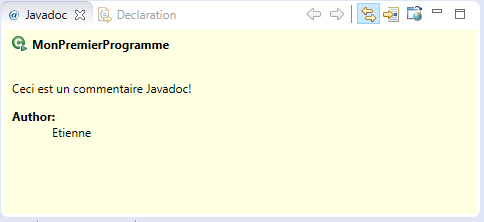
\includegraphics[scale=1]{javadoc-eclipse.png}
	\caption{Visualisation de la Javadoc dans Eclipse}
\end{figure}
%
%
La Javadoc possède plusieurs attributs spéciaux débutant par un arrobe \commande{@}. Les exemples de ce guide feront appel aux trois attributs suivants.

\begin{labeling}{@author\ }

\item[\textbf{@author}] On l'utilise dans l'entête d'une classe pour en spécifier l'auteur.
\item[\textbf{@param}] Dans l'entête de méthodes, il précise le rôle de chaque paramètre.
\item[\textbf{@return}] Également dans l'entête de méthodes, il précise la valeur de retour.

\end{labeling}
%





%----------------------------------------------------
%
%
% Chapitre 3 - Variables et opérateurs
%
%
%----------------------------------------------------
\chapter{Variables et opérateurs}

\textit{Manuel de référence : p. 23 à 32.}

%--------------------------------------------------------
% Section - Déclaration
%--------------------------------------------------------
%
\section{La déclaration de variables}
%
Une \textbf{variable} est une case mémoire pouvant contenir un certain type de données. Comme son nom l'indique, sa valeur est \emph{variable} : elle peut changer au cours l'exécution.

\begin{figure}[!ht]
	\centering
	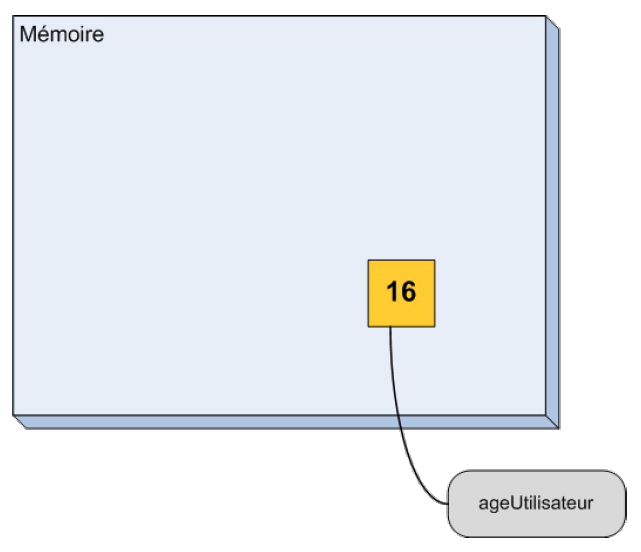
\includegraphics[scale=0.75]{variable-memoire.png}
	\caption{Une variable contenant l'âge de l'utilisateur en mémoire.}
\end{figure}

Pour commencer, regardons un programme utilisant une variable de type \emph{String}.

\begin{MyTCB}{Utilisation d'une variable String}
/**
 * Affiche des noms dans la console.
 * 
 * @author Etienne
 */
public class AffichageNom {

	public static void main(String[] args) {
		
		String nom = "Étienne"; // Nom de l'utilisateur
		
		System.out.println("Je m'appelle " + nom + "!"); //Affichage
		
		nom = "Alexandre"; //Nouvelle valeur
		
		System.out.println("Je m'appelle maintenant " + nom + "!"); //Affichage de la nouvelle valeur
		
	}

}
\end{MyTCB}

\begin{tcolorbox}[title={Sortie console}, sharp corners = south, boxsep = 1.5mm] \tt
	Je m'appelle Étienne!\\
	Je m'appelle maintenant Alexandre!
\end{tcolorbox}

On commence par créer la variable \texttt{nom} de type \emph{String} et on lui donne la valeur \texttt{"Étienne"}. Pour mettre une valeur dans une variable, on utilise le signe égal \commande{=}. L'affectation se fait toujours \textbf{de la droite vers la gauche ($\boldsymbol{\Leftarrow}$)}. On affiche ensuite la valeur de \texttt{nom} dans la console. À la troisième instruction, on met la valeur \texttt{"Alexandre"} dans \texttt{nom}. L'ancienne valeur est alors \textbf{écrasée} par la nouvelle. La dernière instruction affiche la nouvelle valeur de \texttt{nom} dans la console.


% Déclaration de variables
%
\begin{tcolorbox}[enhanced,colframe=ultRed,
	title={Déclaration et initialisation de variables},
	sharp corners=south,
	boxsep = 1.5mm]
Déclaration et initialisation ($\Leftarrow$) dans la même instruction\\
\texttt{\color{ultRed} type} \texttt{\color[RGB]{255, 34, 12} nomVariable} = \texttt{\color[RGB]{63, 136, 197} valeur};%
%
\tcblower
%
Déclaration, puis affectation ($\Leftarrow$) d'une valeur  plus tard dans le programme\\
\texttt{\color{ultRed} type} \texttt{\color[RGB]{255, 34, 12} nomVariable};\\
...\\
\texttt{\color[RGB]{255, 34, 12} nomVariable} = \texttt{\color[RGB]{63, 136, 197} valeur};
\end{tcolorbox}


Lorsque c'est possible, on déclare et on initialise une variable en même temps. C'est ce qui a été fait dans l'exemple précédent. Lorsqu'on ne connaît pas quelle valeur lui donner, on peut la déclarer et lui donner une valeur plus tard.

On peut donner n'importe quel nom à une variable, tant qu'il respecte les conditions suivantes :
\begin{itemize}
	\item pas d'espace ni d'accent;
	\item ne commence pas par un chiffre;
	\item commence par une minuscule;
	\item si son nom est composé de plusieurs mots, les autres mots peuvent commencer par une majuscule.
\end{itemize}

Par exemple, les identificateurs \texttt{prix}, \texttt{ageUtilisateur}, \texttt{vitesseMoteurGauche1} et \texttt{estOuvert} respectent cette convention. 




%--------------------------------------------------------
% Section - Lire console
%--------------------------------------------------------
%
\section{Lire la console}
%
Vous savez déjà comment afficher du texte dans la console avec la méthode \texttt{System.out.println()}. Par contre, il pourrait être pratique de lire ce qui est écrit dans la console. Pour effectuer cette tâche, nous utiliserons la class \texttt{Scanner} de la manière suivante.

% Code Scanner
%
\begin{MyTCB}{Demander et afficher un nom}
import java.util.Scanner;

/**
 * Demande le nom de l'utilisateur, puis l'affiche.
 * 
 * @author Etienne
 */
public class DemanderNom {

	public static void main(String[] args) {
		
		String nom;
		Scanner scanner = new Scanner(System.in);
		
		//Demander le nom
		System.out.print("Saisissez votre nom : ");
		nom = scanner.nextLine();
		
		//Affichage
		System.out.println("Votre nom est " + nom + "!");

	}

}
\end{MyTCB}

\begin{console}
Saisissez votre nom : {\color{blue} Étienne}\\
Votre nom est Étienne!
\end{console}
Ici, on déclare une variable sans l'initialiser. C'est tout à fait logique, car on ne connaît pas encore le nom à afficher. On déclare ensuite une variable spéciale : la variable \texttt{scanner} de type \texttt{Scanner}. C'est elle qui va nous permettre de lire les entrées dans la console. Remarquez son initialisation : on utilise le \commande{new} suivi de \texttt{Scanner}, le type de notre variable. Nous verrons plus loin que c'est parce que \commande{scanner} est un \textbf{objet}, une sorte de « super-variable ». 

Par la suite, on utilise une variante de \texttt{println()} : la méthode \texttt{print()}. Elles agissent presque de la même façon, sauf que \texttt{print()} n'ajoute pas de saut de ligne après avoir affiché le texte. Essayez les deux et constatez la différence.

Ensuite, on utilise notre \texttt{scanner} et on appelle sa méthode \texttt{nextLine()}. Cela indique au programme de faire une pause jusqu'à ce qu'on écrive un mot dans la console et qu'on appuie sur la touche \commande{Entrée}. Le texte saisi est ensuite stocké dans la variable \texttt{nom} grâce à l'opérateur \commande{=}.

Finalement, on affiche la valeur de \texttt{nom} par concaténation avec d'autres chaînes de caractères. 


%--------------------------------------------------------
% Section - Types primitifs
%--------------------------------------------------------
%
\section{Les variables de type primitif}
%
Jusqu'à présent, nous avons uniquement déclaré des variables de type \texttt{String} et \texttt{Scanner}. Ces variables sont en vérité des \textbf{objets}. Nous verrons plus tard ce que cela signifie. Il existe cependant des types de variables qui sont à la base de tout : les types primitifs. 

\begin{center}
	\renewcommand{\arraystretch}{1.5}
	\begin{tabular*}{\linewidth}{@{\extracolsep{\fill} } l l l} \toprule
		\textbf{Type} & \textbf{Ce qu'il contient} & \textbf{Exemple} \\ \midrule
		\texttt{int} & Un nombre entier. & \texttt{int ageUtilisateur = 20;} \\
		\texttt{double} & Un nombre à virgules de précision double. & \texttt{double prix = 19.95;} \\
		\texttt{boolean} & Une valeur booléenne (\textbf{true} ou \textbf{false}). & \texttt{boolean estOuvert = true;} \\ \bottomrule
	\end{tabular*}
	\captionof{figure}{Les types primitifs les plus utilisés.}
\end{center}

Ces types débutent par une minuscule puisqu'ils sont primitifs, alors que \texttt{String} et \texttt{Scanner} débutent par une majuscule puisqu'ils représentent une classe d'objets. 

\begin{MyTCB}{Affichage de variables primitives}
/**
 * Affiche des données de type primitif.
 * 
 * @author Etienne
 */
public class AffichagePrimitif {

	public static void main(String[] args) {
		
		int age = 14, ageAmi = 13;
		double taille = 1.45;
		
		System.out.println("J'ai " + age + " ans!");
		System.out.println("Mon ami a " + ageAmi + " ans.");
		System.out.println("Je mesure " + taille + " m.");

	}

}
\end{MyTCB}

\begin{tcolorbox}[title={Sortie console}, sharp corners = south, boxsep = 1.5mm] \tt
	J'ai 14 ans!\\
	Mon ami a 13 ans.\\
	Je mesure 1.45 m.
\end{tcolorbox}

À la ligne 10, on déclare deux variables du même type sur la même ligne. C'est tout à fait légal, il suffit de séparer leurs noms par des virgules.

Avant un \texttt{Scanner}, il est également possible d'obtenir des données de type primitif à partir de la console.

\begin{MyTCB}{Demande de l'âge et de la taille}
import java.util.Scanner;

/**
 * Demande l'âge et la taille de l'utilisateur,
 * puis l'affiche dans la console.
 * 
 * @author Etienne
 */
public class AgeTaille {

	public static void main(String[] args) {
		
		int age;
		double taille;
		Scanner scanner = new Scanner(System.in);
		
		//Demande de l'âge
		System.out.print("Saisissez votre âge : ");
		age = scanner.nextInt();
		
		//Demande de la taille
		System.out.print("Saisissez votre taille : ");
		taille = scanner.nextDouble();
		
		//Affichage
		System.out.println("Vous avez " + age + " ans et mesurez " + taille + " m.");

	}

}
\end{MyTCB}
\begin{console}
	Saisissez votre âge : {\color{blue} 20}\\
	Saisissez votre taille : {\color{blue} 1,80} \\
	Vous avez 20 ans et mesurez 1.8 m.
\end{console}

Tout comme \texttt{nextLine()}, les méthodes \texttt{nextInt()} et \texttt{nextDouble()} attendent qu'une valeur soit saisie dans la console. Elles retournent ensuite ces valeurs pour qu'elles puissent être stockées dans des variables de notre choix.


\section{Les constantes}

Jusqu'à présent, une variable agit comme une case dans laquelle on range une donnée pour pouvoir y faire référence plus tard. Cette valeur peut changer au cours du programme. Cependant, dans certains cas, on peut vouloir que le contenu d'une variable ne puisse pas changer. C'est ce qu'on appelle une \textbf{constante}.

% Déclaration de constantes
%
\begin{tcolorbox}[enhanced,colframe=ultRed,
	title={Déclaration de constantes},
	sharp corners=south,
	boxsep = 1.5mm]
Utilisation du mot-clé \textbf{final}\\
\texttt{final {\color{ultRed}type}} \texttt{\color[RGB]{255, 34, 12} NOM{\_}CONSTANTE} = \texttt{\color[RGB]{63, 136, 197} valeur};%
\end{tcolorbox}

Il suffit d'ajouter le mot-clé \texttt{final} devant la déclaration pour transformer une variable en constante. Il est alors impossible de redéfinir sa valeur. Par convention, le nom d'une constante est écrit tout en majuscules. On utilise alors la barre de soulignement pour séparer les différents mots.

\begin{code}
	final double NOMBRE_NIVEAUX = 10; //Constante
NOMBRE_NIVEAUX = 12; // Le compilateur affiche une erreur!
\end{code}

Les constantes sont très utiles pour les valeurs qui changent rarement et qui sont utilisées à plusieurs endroits. Si cette valeur doit être modifiée, il suffit alors de la changer à un endroit et le tour est joué!



\section{Les opérateurs arithmétiques}

Maintenant que l'on peut stocker des nombres dans des variables, voyons comment effectuer des opérations arithmétiques sur ceux-ci. La priorité des opérations s'applique.

\begin{center}
\begin{tabularx}{0.5\linewidth}{X c} \toprule
\textbf{Opération} & \textbf{Symbole} \\ \midrule
Addition & + \\
Soustraction & - \\
Multiplication & * \\
Division & / \\
Modulo {\footnotesize (reste de la division)} & \% \\ \bottomrule
\end{tabularx}
\captionof{figure}{Les opérateurs arithmétiques.}
\end{center}

\begin{MyTCB}{Années avant la majorité}
import java.util.Scanner;

/**
 * Demande l'âge de l'utilisateur et affiche le nombre
 * d'années avant qu'il soit majeur.
 * 
 * @author Etienne
 */
public class Majorite {

	public static void main(String[] args) {
		
		int age;
		final int AGE_MAJORITE = 18; // L'âge de la majorité est fixe
		Scanner scanner = new Scanner(System.in);
		
		//Demander l'âge
		System.out.print("Saisissez votre âge : ");
		age = scanner.nextInt();
		
		//Âge avant majorité
		System.out.println("Vous serez majeur dans " + (AGE_MAJORITE - age) + " ans.");

	}

}
\end{MyTCB}
\newpage

\begin{MyTCB}[breakable]{Liquidation d'un inventaire}
import java.util.Scanner;

/**
 * Gestion de la liquidation
 * d'un inventaire.
 * 
 * @author Etienne
 */
public class Liquidation {

	public static void main(String[] args) {
		
		int joursRestants; // Nombre de jours avant la fermeture
		
		int nombreItems; // Nombre d'items restants en inventaire
		double prixItem; // Prix d'un item
		double prixTotal; // Prix d'un item avec les taxes
		double valeurInventaire; // Valeur de tous les items
		
		final double TAXES = 1.15; // Taxes fixes de 15%
		
		Scanner scanner = new Scanner(System.in);
		
		
		// Nombre de jours restants
		System.out.print("Nombre de jours avant la fermeture : ");
		joursRestants = scanner.nextInt();
		
		// Nombre d'items
		System.out.print("Nombre d'items restants : ");
		nombreItems = scanner.nextInt();
		
		// Prix d'un item
		System.out.print("Prix d'un item : ");
		prixItem = scanner.nextDouble();
		
		// Prix total d'un item
		prixTotal = prixItem * TAXES;
		
		// Valeur de l'inventaire
		valeurInventaire = prixItem * nombreItems;
		
		// Affichage
		System.out.println("Le prix à payer avec taxes est de " + prixTotal + "$.");
		System.out.println("Votre inventaire vaut " + valeurInventaire + "$.");
		System.out.println("Pour tout liquider, vous devrez vendre environ " + (nombreItems / joursRestants) + " items par jour.");
		
	}
}
\end{MyTCB}
%
\begin{console}
Nombre de jours avant la fermeture : {\color{blue} 10}\\
Nombre d'items restants : {\color{blue} 50}\\
Prix d'un item : {\color{blue} 11,40}\\
Le prix à payer avec taxes est de 13.11\$.\\
Votre inventaire vaut 570.0\$.\\
Pour tout liquider, vous devrez vendre environ 5 items par jour.
\end{console}

Dans les deux exemples précédents, on effectue des calculs avant l'affectation d'une variable ou directement dans un \texttt{println()} pour afficher le résultat. Les deux sont acceptables, tant que le code reste clair et que les parenthèses sont placées aux bons endroits. Dans le cas de calculs longs et compliqués, il est préférable de les isoler pour que ce soit plus lisible.

\section{Les opérateurs d'affectation}
Vous connaissez déjà l'opération d'affectation de base : le symbole égal \commande{=}. C'est le plus commun. Il existe cependant des raccourcis qui peuvent être utiles dans plusieurs cas. Dans tous les cas, l'affectation se fait toujours \textbf{de la droite vers la gauche ($\boldsymbol{\Leftarrow}$)}.

\begin{center}
\renewcommand{\arraystretch}{1.5}
	\begin{tabularx}{\linewidth}{l c X X} \toprule
		\textbf{Rôle} & \textbf{Symbole} & \textbf{Exemple} & \textbf{Équivalent} \\ \midrule
		Ajout de... & \texttt{+=} & \texttt{age += 2;} & \texttt{age = age + 2;} \\
		Retrait de... & \texttt{-=} & \texttt{vie -= dommages;} & \texttt{vie = vie - dommages;} \\
		Multiplier par... & \texttt{*=} & \texttt{prix *= rabais;} & \texttt{prix = prix * rabais;} \\
		Diviser par... & \texttt{/=} & \texttt{taille /= 3.28;} & \texttt{taille = taille / 3.28;} \\
		Incrémentation & \texttt{++} & \texttt{compteur++;} & \texttt{compteur += 1;} \\
		Décrémentation & \texttt{-{}-} & \texttt{points-{}-;} & \texttt{points -= 1;} \\ \bottomrule
	\end{tabularx}
	\captionof{figure}{Les opérateurs d'affectation.}
\end{center}


\section{La librairie \texttt{Math}}
Java a une librairie standard très fournie. Elle comprend, entre autres, la classe \texttt{Math}. Celle-ci fournit plusieurs fonctions mathématiques de base : 
\begin{itemize}
	\item la valeur absolue (\texttt{abs}),
	\item les exposants (\texttt{pow}),
	\item les fonctions trigonométriques (\texttt{sin}, \texttt{cos}, \texttt{tan}, etc.),
	\item le maximum et le minimum (\texttt{max} et \texttt{min}),
	\item la racine carrée (\texttt{sqrt}),
	\item l'arrondi (\texttt{round}, \texttt{ceil} et \texttt{floor}).
\end{itemize}

\begin{MyTCB}{Utilisation de la classe Math}
import java.util.Scanner;

/**
 * Affiche la valeur absolue et le cube d'un nombre.
 * 
 * @author Etienne
 *
 */
public class TestMath {

	public static void main(String[] args) {
		
		double nombre;
		Scanner scanner = new Scanner(System.in);
		
		//Obtention du nombre
		System.out.print("Saisissez un nombre : ");
		nombre = scanner.nextDouble();
		
		//Calculs
		System.out.println("\nLa valeur absolue du nombre est : " + Math.abs(nombre));
		System.out.println("Le cube du nombre est : " + Math.pow(nombre, 3));

	}

}
\end{MyTCB}

La méthode \texttt{pow()} prend deux paramètres : le premier est la base et le deuxième est l'exposant. Ainsi, \texttt{pow(x, y)} $= x^y$.




%----------------------------------------------------
%
%
% Chapitre 4 - Instructions conditionnelles
%
%
%----------------------------------------------------
\chapter{Les instructions conditionnelles}

\textit{Manuel de référence : p. 39 à 46.}

\section{Le \textit{if else}}
Jusqu'à présent, vos programmes se sont exécutés de manière \textbf{séquentielle} : toutes les instructions sont exécutées les unes après les autres. En réalité, il est bien rare qu'un programme suive une seule séquence. Avec les \textbf{instructions conditionnelles}, il sera possible d'exécuter une certaine partie de votre programme uniquement si une certaine condition est respectée. Nous utiliserons alors le \emph{if else}.

\begin{tcolorbox}[enhanced,colframe=ultRed,
	title={La structure \emph{if else}},
	sharp corners=south,
	boxsep = 1.5mm]
\texttt{{\color{ultRed}if} (} {\color[RGB]{255, 34, 12} condition} \texttt{) \{}\\
	\hspace*{0.5cm} {\color[RGB]{63, 136, 197} instruction1};\\	
	\hspace*{0.5cm} ... \texttt{// Si la condition est vraie...}\\
\texttt{\}\\
{\color{ultRed} else} \{ // Facultatif \\}
	\hspace*{0.5cm} {\color[RGB]{63, 136, 197} instruction2};\\ 
	\hspace*{0.5cm} ... \texttt{// Si la condition est fausse...} \\
\texttt{\}}
%
\end{tcolorbox}

Si la condition donnée est vraie, alors les instructions contenues dans le premier bloc seront exécutées. Sinon, ce sont celles du deuxième bloc qui seront exécutées. Le \emph{else} est facultatif. S'il n'y a pas de \emph{else} et que la condition est fausse, alors le programme continu son exécution normalement, sans exécuter le contenu du \emph{if}.

Comme une condition peut être vraie ou fausse, on dit que c'est une condition \textbf{booléenne}. C'est d'ailleurs une des principales utilités du type \texttt{boolean}.



\section{Les opérateurs de comparaison et les opérateurs logiques}

Pour exprimer une condition, on peut utiliser les \textbf{opérateurs de comparaison} et les \textbf{opérateurs logiques}. Les principaux sont les suivants.

\begin{center}
\renewcommand{\arraystretch}{1.5}
	\begin{tabularx}{0.8\linewidth}{l c X X} \toprule
		\textbf{Rôle} & \textbf{Symbole} & \textbf{Exemple} \\ \midrule
		égal & \texttt{==} & \texttt{a == 2} \\
		n'est pas égal & \texttt{!=} & \texttt{prix != 10} \\
		est plus grand & \texttt{>} & \texttt{rabais > prix} \\
		est plus grand ou égal & \texttt{>=} & \texttt{age >= AGE\_MAJORITE} \\
		est plus petit & \texttt{<} & \texttt{rotation < 25.1} \\
		est plus petit ou égal & \texttt{<=} & \texttt{distance <= 120} \\
		ou & \texttt{||} & \texttt{a == 10 || b == 5} \\
		et & \texttt{\&\&} & \texttt{distance >= 10 \&\& angle == 180} \\
		n'est pas & \texttt{!} & \texttt{!estOuvert} \\ \bottomrule
	\end{tabularx}
	\captionof{figure}{Les opérateurs de comparaison et les opérateurs logiques.}
\end{center}

Les six premiers sont appelés les \textbf{opérateurs de comparaison}. On les utilise pour comparer des nombres ensemble. Les trois derniers sont appelés les \textbf{opérateurs logiques}. Ils permettent de modifier d'autres conditions ou booléens. Avec le \textbf{ou}, la nouvelle condition est vraie si la première ou la deuxième condition est vraie. Quant au \textbf{et}, il faut que les deux conditions soient vraies pour que la nouvelle condition soit vraie. Finalement, le dernier opérateur permet d'inverser une valeur booléenne. 


\begin{MyTCB}{Validation d'une année de naissance}
import java.util.Calendar;
import java.util.Scanner;
/**
 * Validation d'une année de naissance.
 * 
 * @author Etienne
 */
public class ValidationNaissance {

	public static void main(String[] args) {
		
		int annee;
		final int ANNEE_MINIMALE = 1900;
		final int ANNEE_COURANTE = Calendar.getInstance().get(Calendar.YEAR); //2017
		Scanner scanner = new Scanner(System.in);
		
		
		//Obtention de l'année
		System.out.print("Saisissez une année de naissance : ");
		annee = scanner.nextInt();
		
		
		//Validation
		if(annee >= ANNEE_MINIMALE && annee <= ANNEE_COURANTE) {
			System.out.println("Année valide.");
		}
		else {
			System.out.println("L'année " + annee + " est invalide.");
			System.out.println("Vous devez recommencer!");
		}

	}

}
\end{MyTCB}

\section{Les \textit{else if} multiples}


\part{La programmation orientée objet}


\part{La librairie WPILib}

\chapter{La classe \texttt{TimedRobot}}

\section{Création d'un projet}
Jusqu'à présent, le coeur de vos programmes se trouvait dans la méthode \texttt{main}. Cependant, le comportement d'un robot est plus complexe qu'une simple méthode. Vos prochains programmes auront comme base la classe \texttt{Robot}, héritant de \texttt{TimedRobot}.

\begin{enumerate}
	\item Dans Eclipse, débutez la création d'un nouveau projet avec \commande{File > New > Other...}, puis, dans le dossier \commande{WPILib Robot Java Project}, sélectionnez \commande{Robot Java Project}.
	\item Donnez un nom à votre projet (débutant avec une lettre majuscule).
	\item Sélectionnez \commande{Command-Based Robot}ou \commande{Timed Robot}, selon le paradigme que vous souhaitez utiliser. Cliquez sur \commande{Finish}.
\end{enumerate}

Vous vous retrouverez ainsi avec un fichier \commande{Robot.java} contenant le squelette d'un programme pour la FRC.

\section{Les méthodes \texttt{Init} et \texttt{Periodic}}

La classe qu'Eclipse a générée pour vous contient déjà quelques méthodes prédéfinies. Chacune d'entre elles a un rôle bien précis.

\tikzset{>={Stealth[scale=1.3,angle'=45]}}
\begin{figure}
\begin{center}
\begin{tikzpicture}[every node/.style = {shape=rectangle, rounded corners, fill=gray!50, draw, minimum width=3.25cm, minimum height=0.8cm, }]

\node (robotInit) at (0,5) {robotInit};
\node (disabledInit) at (0,3) {disabledInit};
\node (disabledPeriodic) at (0,1) {disabledPeriodic};
\node (autonomousInit) at (4.5,3) {autonomousInit};
\node (autonomousPeriodic) at (4.5,1) {autonomousPeriodic};
\node (teleopInit) at (9,3) {teleopInit};
\node (teleopPeriodic) at (9,1) {teleopPeriodic};
\node (testInit) at (13.5,3) {testInit};
\node (testPeriodic) at (13.5,1) {testPeriodic};

\node (periode) [fill=white] at (6.75, 5) {Changement de période};

\draw[fill] (0,7) circle [radius=0.25];

\draw[->, to path={-- (\tikztotarget)}] (0,7) edge (robotInit) (robotInit) edge (disabledInit) (disabledInit) edge (disabledPeriodic) (autonomousInit) edge (autonomousPeriodic) (teleopInit) edge (teleopPeriodic) (testInit) edge (testPeriodic);
\draw[->] (-1.0,1.5) arc [radius=0.7, start angle=45, end angle= 315];
\draw[->] (3.25,1.5) arc [radius=0.7, start angle=45, end angle= 315];
\draw[->] (8.0,1.5) arc [radius=0.7, start angle=45, end angle= 315];
\draw[->] (12.5,1.5) arc [radius=0.7, start angle=45, end angle= 315];
\draw (disabledPeriodic) edge ++(0,-1.5) (autonomousPeriodic) edge ++(0,-1.5) (teleopPeriodic) edge ++(0,-1.5) (testPeriodic) edge ++(0,-1.5);
\draw (0,-0.5) -| (16,5);
\draw[->] (16,5) -- (9.1, 5);
\draw (periode) edge (6.75, 4);
\draw[->] (6.75, 4) -| (1.0,3.4);
\draw[->] (6.75, 4) -| (4.5,3.4);
\draw[->] (6.75, 4) -| (9,3.4);
\draw[->] (6.75, 4) -| (13.5,3.4);
\end{tikzpicture}
\caption{Séquence d'éxécution des méthodes de la classe Robot.}
\end{center}
\end{figure}

Chaque état dans lequel peut être le robot possède sa méthode \texttt{Init} et \texttt{Periodic}. Par exemple, lorsque le robot entre en période autonome, le contenu de la méthode \texttt{autonomousInit} est appelé une fois. Ensuite, la méthode \texttt{autonomousPeriodic} est appelée en boucle (périodiquement, soit environ aux 20 millisecondes) tant que le robot reste dans cet état.  

La seule exception est la méthode \texttt{robotInit} : elle s'exécute une fois, au tout début, lorsque le programme démarre. Habituellement, on y initialise les différentes composantes du robot, ses sous-systèmes, etc.

\section{Faire avancer le robot}

\begin{MyTCB}{Utilisation de DifferentialDrive avec Joystick}
public class MonPremierRobot extends TimedRobot {
	
	private VictorSP moteurGauche, moteurDroit;
	private DifferentialDrive basePilotable;
	private Joystick joystick;
	
	@Override
	public void robotInit() {
		moteurGauche = new VictorSP(0);
		moteurDroit = new VictorSP(1);
		basePilotable = new DifferentialDrive(moteurGauche, moteurDroit);
		joystick = new Joystick(0);
	}
	
	@Override
	public void autonomousPeriodic() {
		moteurGauche.set(0.5);
		moteurDroit.set(-0.5);
	}
	
	
	@Override
	public void teleopPeriodic() {
		basePilotable.arcadeDrive(-1 * joystick.getY(), joystick.getX());
	}

}

\end{MyTCB}

Dans un premier temps, on déclare comme attributs privés de classe les composantes de notre robot : deux contrôleurs moteur \texttt{VictorSP}, une \text{DifferentialDrive} et un \texttt{Joystick}. On les instancie dans la méthode \texttt{robotInit}.

Ensuite, en période autonome, on met le moteur gauche à 50 \% de sa puissance vers à l'avant, et le moteur droit, à 50 \% vers l'arrière. Le robot tournera donc en rond pendant 15 secondes.

Finalement, en période téléopérée, on utilise la méthode \texttt{arcadeDrive} avec le Joystick pour contrôleur le robot naturellement. 

\subsection{La classe \texttt{VictorSP}}
Cette classe sert à déclarer des contrôleurs moteur de type VictorSP. Des classes existent pour chaque modèle de contrôleur moteur : Talon, Spark, Jaguar, etc.

Son constructeur reçoit en paramètre un nombre entier (voir lignes 9 et 10). Il s'agit du port PWM du RoboRIO où est branché le contrôleur.

Cette classe possède la méthode \texttt{set(double)}. Elle reçoit un nombre compris entre -1.0 et 1.0, spécifiant la puissance à laquelle le moteur doit aller.

\subsection{La classe \texttt{DifferentialDrive}}

Cette classe fournit plusieurs méthodes utiles pour contrôler la base pilotable. Bien qu'il serait possible de calculer manuellement les valeurs à envoyer à chaque moteur, il est plus pratique (et rapide) d'utiliser cette classe. Elle est configurée pour les bases pilotables de type « tank ». Les classes \texttt{MecanumDrive} et \texttt{KilloughDrive} (robot à trois roues) sont également disponibles.

Le constructeur reçoit comme arguments les deux contrôleurs moteur : celui de gauche et celui de droite. La \texttt{DifferentialDrive} doit les avoir en référence pour contrôler la base pilotable.

Sa méthode \texttt{arcadeDrive(double, double)} reçoit deux nombres en paramètre : \texttt{forward} et \texttt{rotation}. Le paramètre \texttt{forward} (entre -1.0 et 1.0) représente la vitesse d'avancée en ligne droite. Le paramètre \texttt{rotation} (entre -1.0 et 1.0) représente la vitesse de rotation, où les valeurs positives vont vers la droite (sens horaire). 

\subsection{La classe \texttt{Joystick}}

On utilise évidemment cette classe pour lire les valeurs d'un Joystick. Son constructeur reçoit en paramètre l'ordre de branchement du Joystick dans la DriverStation (à partir de 0). Cet ordre est très important lorsque le robot est contrôlé par plus d'une manette en même temps.

On accède aux valeurs des axes (de -1.0 à 1.0) avec la méthode \texttt{getRawAxis(int)}, où l'entier en paramètre est le numéro de l'axe (à partir de 0). Des raccourcis existent pour les axes principaux : \texttt{getX()} et \texttt{getY()}. Cependant, l'axe des Y est inversé selon notre logique : il renvoie -1.0 lorsqu'on pousse le Joytick vers l'avant, et 1.0 lorsqu'on le tire vers soi. On multiplie donc cette valeur par -1 avant de l'envoyer comme paramètre \texttt{forward} à \texttt{arcadeDrive} (voir ligne 24).

L'état des boutons est donné par la méthode \texttt{getRawButton(int)}, où l'entier en paramètre est le numéro du bouton (à partir de 1). La méthode renvoie le booléen \texttt{\bfseries true} si le bouton est appuyé, et \texttt{\bfseries false} dans le cas contraire.


\end{document}


